%! Author = Wiktor Rostkowski, Mateusz Budzisz
%! Date = 29/04/2024

\chapter{Testy}
\label{ch:testy}

\section{Testy jednostkowe}
\label{sec:testy-jednostkowe}
W naszej pracy inżynierskiej zastosowaliśmy GitHub Actions do automatyzacji testów jednostkowych(opisane \pageref{sec:github-actions} ), które przeprowadziliśmy dla różnych komponentów naszego projektu.
Testy jednostkowe były kluczowym elementem, zapewniającym jakość i niezawodność naszego oprogramowania. 
W sumie przeprowadziliśmy 638 testów, obejmujących frontend, backend oraz dokumentację.\newline

\indent W ramach projektu frontend wykonaliśmy 151 testów jednostkowych, koncentrując się na każdym komponencie aplikacji. Testy te obejmowały funkcjonalności poszczególnych 
komponentów, sprawdzając ich poprawne renderowanie, interakcje użytkownika oraz walidację danych. Głównym celem było zapewnienie, że każdy komponent działa zgodnie z założeniami i spełnia swoje funkcje.\newline

\indent Dla backendu obejmował 159 testów jednostkowych, które dotyczyły logiki biznesowej, operacji na danych oraz interakcji z bazą danych. 
Testowaliśmy funkcje oraz metody, aby upewnić się, że zwracają one poprawne wyniki w różnych scenariuszach. Dodatkowo sprawdzaliśmy poprawność integracji wszystkich zależności i usług zewnętrznych.\newline

\indent Na potrzeby projektu dokumentacja przeprowadziliśmy 328 testów jednostkowych, które miały na celu weryfikację poprawności oraz kompletności dokumentacji technicznej i użytkowej.
 Sprawdzaliśmy, czy wszystkie przykłady kodu działają poprawnie i czy dokumentacja jest aktualna w stosunku do bieżącego stanu projektu. Testy te były kluczowe dla zapewnienia, że dokumentacja 
 jest pomocna i dokładna, wspierając użytkowników i deweloperów w korzystaniu z naszego systemu.\newline

 \indent Podsumowując, przeprowadzenie łącznie 638 testów jednostkowych pozwoliło nam na dogłębne sprawdzenie działania naszej aplikacji na każdym etapie naszej pracy. 
Wykorzystanie GitHub Actions do automatyzacji testów zapewniło efektywność i powtarzalność procesu testowania, co jest kluczowe dla utrzymania wysokiej jakości oprogramowania. 
Dzięki temu podejściu jesteśmy pewni, że nasza aplikacja jest dobrze przetestowana i gotowa do wdrożenia.\newline

\begin{figure}[H]
    \centering
    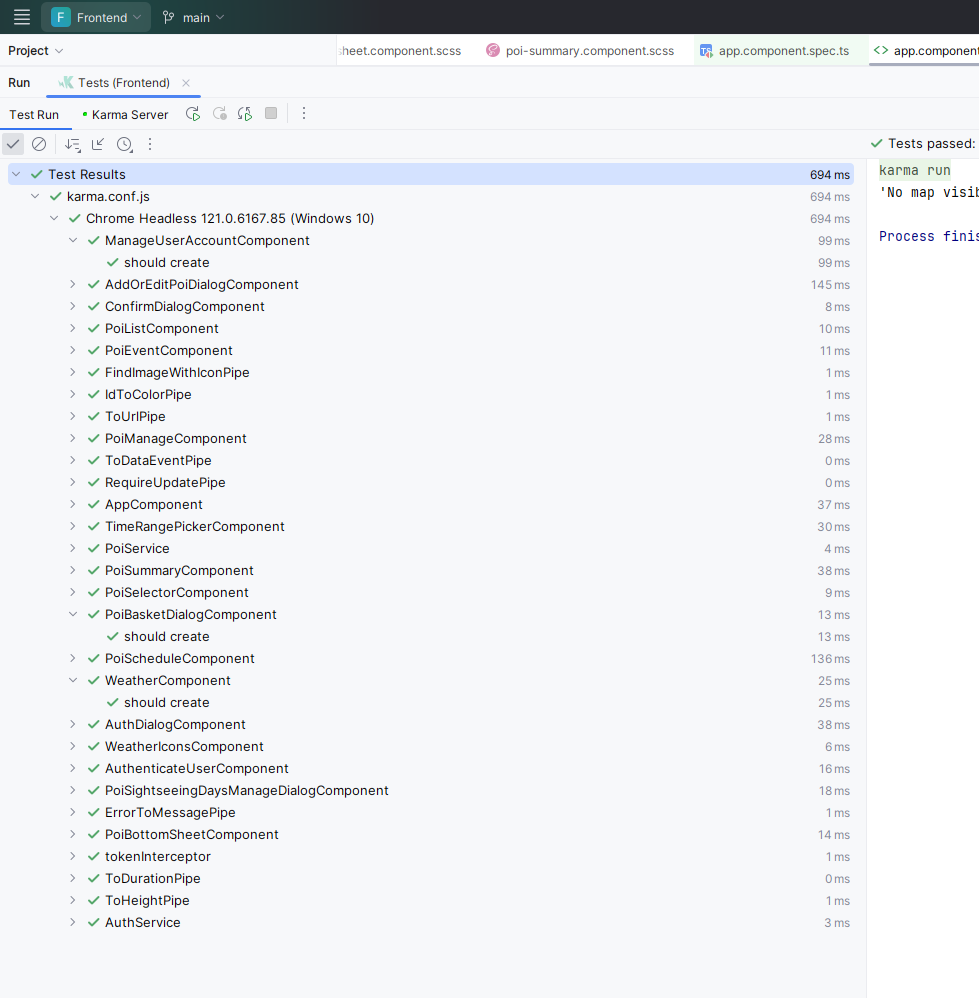
\includegraphics[width=1\textwidth]{attachments/testfrontend}
    \caption{Testy jednostkowe Frontend}
    \label{fig:testfronted}
\end{figure}

\section{Testy wydajnościowe}
\label{sec:testy-wydajnosciowe}

W ramach naszej pracy inżynierskiej wykonaliśmy testy wydajności za pomocą narzędzia Lighthouse, aby ocenić i poprawić wydajność naszej aplikacji internetowej. \newline
Lighthouse jest narzędziem open-source opracowanym przez Google, które automatycznie ocenia strony internetowe pod kątem wydajności, dostępności, najlepszych praktyk i SEO. \newline
Przeprowadziliśmy testy zarówno dla wersji mobilnej, jak i desktopowej naszej aplikacji. \newline
Zdecydowaliśmy się na Lighthouse ze względu na jego wszechstronność i precyzję w ocenie kluczowych aspektów wydajnościowych.  \newline
Narzędzie to jest szeroko stosowane w branży i dostarcza szczegółowych raportów, które pomagają zidentyfikować obszary wymagające optymalizacji. \newline
\begin{figure}[H]
    \centering
    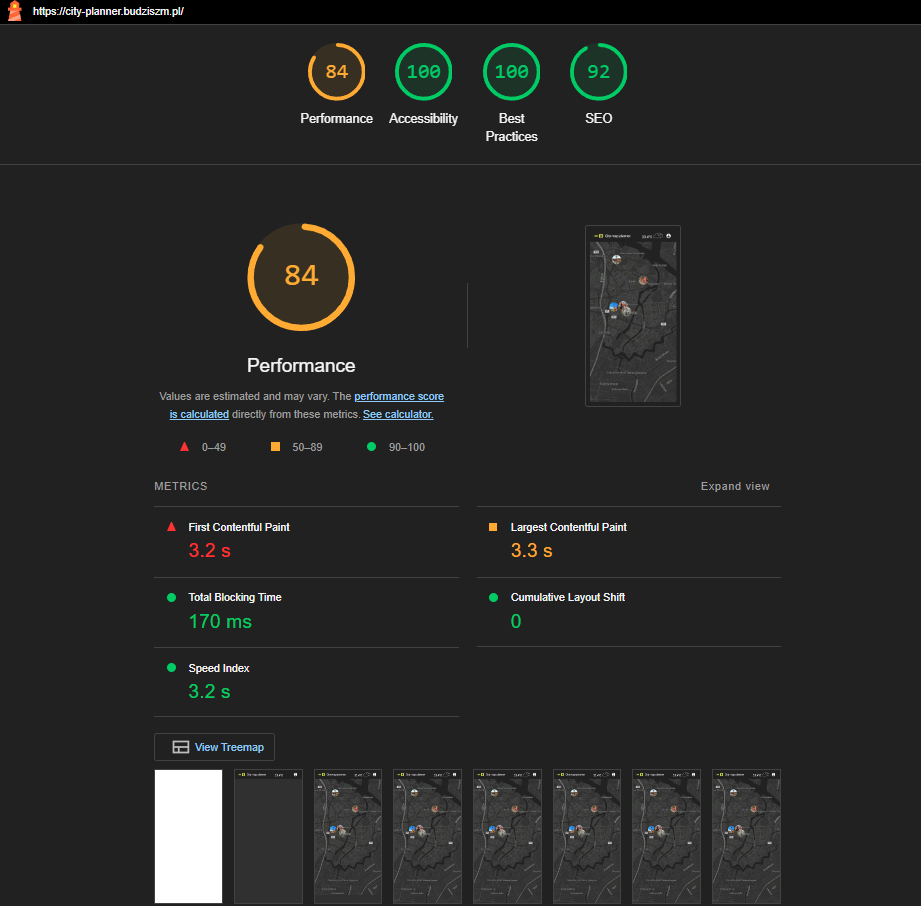
\includegraphics[width=1\textwidth]{attachments/lighthouse-mobile}
    \caption{Widok testu lighthouse mobile}
    \label{fig:testy-dostepnosci}
    \end{figure}

    \begin{figure}[H]
        \centering
        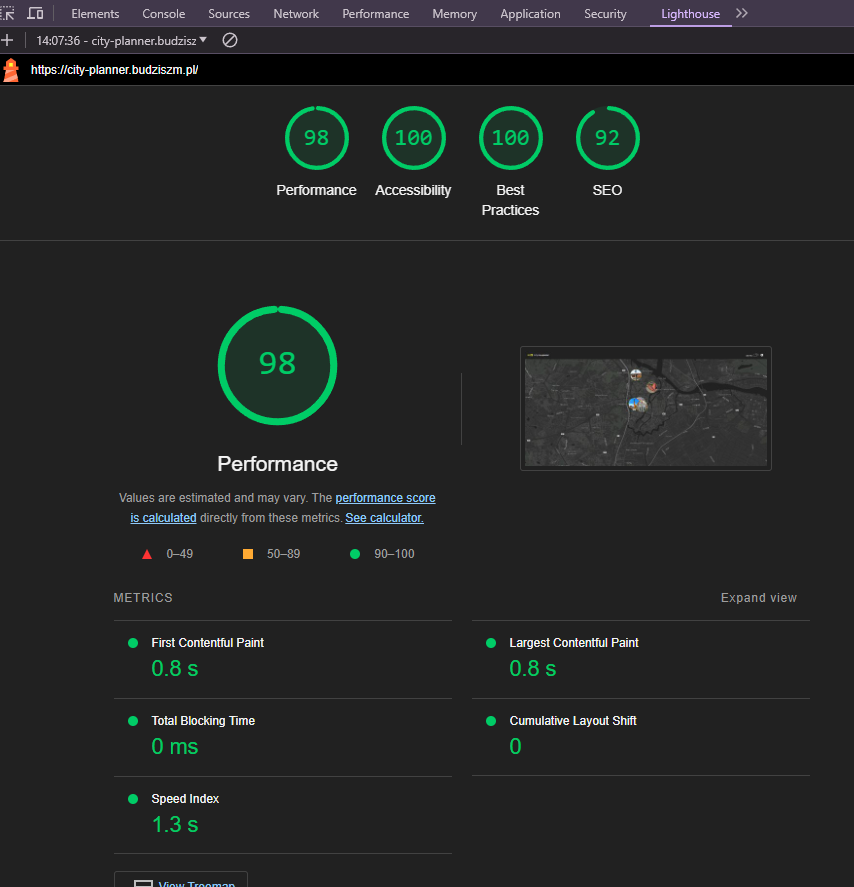
\includegraphics[width=1\textwidth]{attachments/lighthouse}
        \caption{Widok testu lighthous komputer}
        \label{fig:testy-dostepnosci}
        \end{figure}
\section{Testy funkcjonalne}
\label{sec:testy-funkcjonalne}

Na koniec każdego przyrostu projektu przeprowadzaliśmy testy funkcjonalne. Za te testy odpowiadała wyznaczona osoba, która nie brała udziału w implementacji danego przyrostu. 
Testy funkcjonalne miały na celu weryfikację działania konkretnej funkcjonalności związanej z danym zadaniem. \newline
Dla zadań bezpośrednio związanych z implementacją user story lub wymagania niefunkcjonalnego, testy przeprowadzano zgodnie z ustalonymi kryteriami akceptacji. \newline

Jeśli podczas testów wykryto, że wprowadzone zmiany mają negatywny wpływ na inne obszary projektu, zadanie było zwracane do zespołu deweloperskiego w celu dokonania niezbędnych poprawek.
\section{Scenariusze testowe}
\label{sec:scenariusze-testowe}

\begin{testowanie}[label={tab:requirements:testnowy1},caption={Scenariusz wymagania: Logowania}]
    \name{Test1}
    \descr{Testowanie logowania}
    \type{Funkcjonalność}
    \test{WO1,F24}
    \testz{1. Otwórz menu logowania.}{Menu logowania jest wyświetlane.}
    \testy{2. Wprowadź poprawne dane logowania.}{Użytkownik jest zalogowany.}
    \result{Sukces}
    \testX{}
    \testXz{1. Otwórz menu logowania.}{Strona logowania jest wyświetlane.}
    \testXy{2. Wprowadź niepoprawne dane logowania.}{Pojawia się komunikat o błędzie.}
    \resultX{Niepowodzenie}
\end{testowanie}

\begin{testowanie}[label={tab:requirements:testnowy1},caption={Scenariusz wymagania:}]
    \name{Test2}
    \descr{Sprawdzenie możliwości zarządzania PO}
    \type{FO4}
    \test{}
    \testz{1. Zaloguj się jako zwykły użytkownik }{Użytkownik zalogowany}
    \testy{2. Włącz stronę do zarządzania POI}{ Otwarcie panelu zarządznia}
    \result{Niepowodzenie, brak możliwości wczytanie informajci}
    \testX{}
    \testXz{1. Zaloguj się jako administrator}{Administrator zalogowany}
    \testXy{2. Włącz strone do zarzadzania POI}{ Otwarcie panelu zarządznia}
    \resultX{ Panel zarządzania POI załadowany prawidłowo}
\end{testowanie}

\begin{testowanie}[label={tab:requirements:test2},caption={Scenariusz wymagania: Zarządzanie POI}]
    \name{Test3}
    \descr{Test zarządzania POI}
    \type{Funkcjonalność}
    \test{}
    \testz{1. Zaloguj się jako zwykły użytkownik.}{Brak dostępu do zarządzania POI.}
    \testy{2. Zaloguj się jako administrator.}{Możliwość zarządzania POI.}
    \result{Sukces}
\end{testowanie}






\begin{figure}[H]
    \centering
    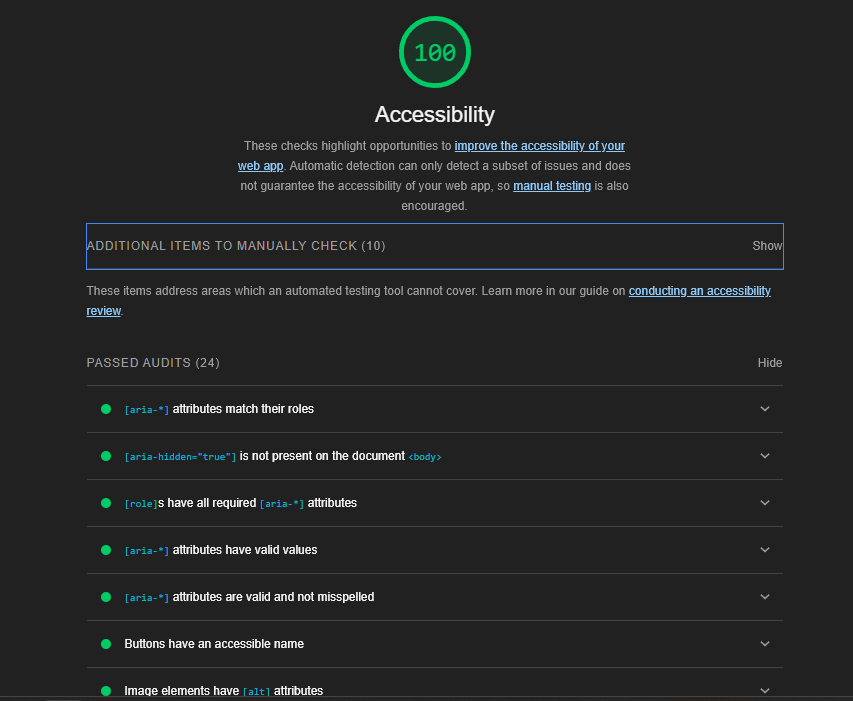
\includegraphics[width=1\textwidth]{attachments/testy-dostepnosci}
    \caption{Widok testu dostępności dla naszej aplikacji}
    \label{fig:testy-dostepnosci}
    \end{figure}